\subsection{问题一求解思路}

场景 A 中每个子图是一个独立 Task。评估程序为每个 Task 重建一张局部计算图：Task 读到但自己不生产的张量，在开头插入一次 COPY\_IN；Task 生产、且被别的 Task 使用或本身是图输出的张量，在结尾插入一次 COPY\_OUT。Task 之间不保留任何核内数据，两个 Task 即使在同一核心上相邻执行也是如此。Task 的激活受两类约束：同核前一个 Task 结束后至少等 $\delta_{\mathrm{same}}=100$ 周期，每个跨核前驱 Task 结束后至少等 $\delta_{\mathrm{cross}}=1000$ 周期。图~\ref{fig:sceneAB}(a) 以三个子图为例画出了这些规则，(b) 为第~\ref{sec:p2-model} 节要用到的场景 B。

\begin{figure}[H]
  \centering
  % 场景 A / B 的 Task 组织与边界搬运对比（3 个子图：s1、s2 在核 0，s3 在核 1；依赖 s1→s2、s1→s3）
\begin{tikzpicture}[x=1mm,y=1mm]
\tikzset{
  sgb/.style={pbox=cB, minimum width=11mm, minimum height=7mm, font=\footnotesize},
  cin/.style={draw=cO, fill=cOL, minimum width=3.2mm, minimum height=7mm, inner sep=0pt, font=\tiny, line width=0.5pt},
  task/.style={draw=ink2, dashed, rounded corners=2pt, inner sep=1.4mm, line width=0.5pt},
  ddr/.style={draw=cG, fill=cGL, minimum height=4mm, font=\scriptsize, text=ink2},
  lab/.style={font=\footnotesize\bfseries, text=ink2, anchor=east},
}
% ======================= (a) 场景 A =======================
\node[font=\small\bfseries, anchor=west] at (-10,25) {(a) 场景 A：每个子图一个 Task};
\node[lab] at (-1,10) {核 0};
\node[lab] at (-1,-10) {核 1};
\node[ddr, minimum width=62mm, anchor=west] (dA) at (0,0) {DDR};
\node[cin] (a1i) at (2,10) {I};
\node[sgb, right=0pt of a1i] (a1) {$s_1$};
\node[cin, right=0pt of a1] (a1o) {O};
\node[task, fit=(a1i)(a1o)] (t1) {};
\node[cin] (a2i) at (36,10) {I};
\node[sgb, right=0pt of a2i] (a2) {$s_2$};
\node[cin, right=0pt of a2] (a2o) {O};
\node[task, fit=(a2i)(a2o)] (t2) {};
\node[cin] (a3i) at (36,-10) {I};
\node[sgb, right=0pt of a3i] (a3) {$s_3$};
\node[cin, right=0pt of a3] (a3o) {O};
\node[task, fit=(a3i)(a3o)] {};
\draw[parrO] (a1o.south) -- ++(0,-7.5) -| (a2i.south);
\draw[parrO] (a1o.south) ++(0,-7.5) -| (a3i.north);
\draw[decorate, decoration={brace, amplitude=2pt}, draw=ink2] ($(t1.north east)+(0.5,1)$) -- node[above=2pt, pnote]{同核等待 $\ge 100$} ($(t2.north west)+(-0.5,1)$);
\node[pnote, text=cO, anchor=east] at ($(a3i.west)+(-3,0)$) {跨核等待 $\ge 1000$};
\node[pnote, anchor=north, text width=64mm, align=left] at (31,-17)
  {同核的 $s_1\to s_2$ 也要写回 DDR 再读入；\\每个 Task 结束都清空核内缓存};
% ======================= (b) 场景 B =======================
\begin{scope}[xshift=76mm]
\node[font=\small\bfseries, anchor=west] at (-10,25) {(b) 场景 B：每核一个 Task};
\node[lab] at (-1,10) {核 0};
\node[lab] at (-1,-10) {核 1};
\node[ddr, minimum width=62mm, anchor=west] (dB) at (0,0) {DDR};
\node[sgb] (b1) at (8,10) {$s_1$};
\node[cin, right=0pt of b1] (b1o) {O};
\node[sgb, right=12mm of b1o] (b2) {$s_2$};
\node[task, fit=(b1)(b1o)(b2)] {};
\draw[parrB] (b1.north) to[bend left=28] node[above, pnote]{L1/UB 驻留} (b2.north);
\node[cin] (b3i) at (36,-10) {I};
\node[sgb, right=0pt of b3i] (b3) {$s_3$};
\node[task, fit=(b3i)(b3)] {};
\draw[parrO] (b1o.south) -- ++(0,-7.5) -| (b3i.north);
\node[pnote, text=cO, anchor=east] at ($(b3i.west)+(-3,0)$) {同步 $+500$};
\node[pnote, anchor=north, text width=62mm, align=left] at (31,-17)
  {同核的 $s_1\to s_2$ 直接复用核内缓存，不产生搬运；\\只有跨核的 $s_1\to s_3$ 经 DDR，并等待 500 周期};
\end{scope}
\end{tikzpicture}

  \caption{场景 A 与场景 B 的 Task 组织与边界搬运（$s_1$、$s_2$ 在核 0，$s_3$ 在核 1；I、O 分别为评估程序插入的 COPY\_IN、COPY\_OUT）}
  \label{fig:sceneAB}
\end{figure}

由这些规则，场景 A 方案的时间代价有四个来源：某个核心计算量明显偏多造成的负载不均衡；跨子图张量写回 DDR 再读入的边界搬运，它还要和其他核心争用 60 bytes/cycle 的总带宽；沿依赖链每经过一次子图边界就要付出的 100 或 1000 周期激活等待；以及子图过大、核内缓存装不下时插入的换入换出。前三项中，后两项随依赖路径上的子图边界增加而变重，而负载均衡和换出又要求子图不能太少、太大。求解思路据此分三步。第一步建立切图与调度的优化模型，把边界搬运和路径上累积的等待写成显式表达式，从中得到“少在依赖链上切分、少跨核”的原则。第二步针对不同结构设计三种构造算法：多分量图按分量装箱，单一巨块图按层级切带，汇聚链结构用通信感知的表调度决定分核、再按换核次数组成子图；三种算法都由构造保证商图无环。第三步对每个（用例，核数）组合在参数网格上生成候选，由官方评估程序选优，再做成组合并、局部搜索和核数补齐三种后处理。整个过程如图~\ref{fig:ladder-p1} 所示，每一步都针对前一步在数据上暴露的不足。

\begin{figure}[H]
  \centering
  % 问题一的求解步骤（5 核平均加速比，数字取自 numbers.tex）
\begin{tikzpicture}[x=1mm,y=1mm]
\def\dx{30}\def\dy{10}
\tikzset{st/.style={pbox=#1, text width=24mm, minimum height=14mm, anchor=south west, font=\footnotesize}}
\node[st=cG] (s0) at (0,0)        {分量装箱\\[1pt]\textbf{\V{p1_k5_lpt_mean}}};
\node[st=cB] (s1) at (\dx,\dy)    {+ 层带划分\\[1pt]\textbf{\V{p1_k5_lptband_mean}}};
\node[st=cB] (s2) at (2*\dx,2*\dy){+ 相位构造\\[1pt]\textbf{\V{ladder_p1_k5_sweep}}};
\node[st=cO] (s3) at (3*\dx,3*\dy){+ 成组合并\\[1pt]\textbf{\V{ladder_p1_k5_coarsen}}};
\node[st=cO, line width=1pt] (s4) at (4*\dx,4*\dy){+ 局部搜索\\+ 核数补齐\\[1pt]\textbf{\V{ladder_p1_k5_monotone}}};
\foreach \i/\j in {0/1,1/2,2/3,3/4} \draw[parrO] (s\i.north) |- (s\j.west);
\tikzset{why/.style={pnote, text=cO, anchor=north, text width=25mm, font=\scriptsize}}
\node[why] at ($(s1.south)+(0,-1)$) {I 类 4 核仅 \V{p1_k4_famI_naive_mean}};
\node[why] at ($(s2.south)+(0,-1)$) {汇聚链跨核依赖多};
\node[why] at ($(s3.south)+(0,-1)$) {同核 Task 过碎};
\node[why] at ($(s4.south)+(0,-1)$) {部分用例多核反慢};
\node[pnote, anchor=north, text width=25mm, font=\scriptsize] at ($(s0.south)+(0,-1)$) {$\alpha=0.25$：\V{p1_k5_naive_mean}};
\draw[-{Stealth[length=2mm]}, line width=0.7pt, draw=ink2] (-3,-12) -- (148,-12) node[pnote, anchor=north east] {评估次数 $\rightarrow$};
\end{tikzpicture}

  \caption{问题一的求解步骤与 5 核平均加速比。框下文字为引入该步的原因，首框下为朴素参数的结果}
  \label{fig:ladder-p1}
\end{figure}

\subsection{问题一模型建立}\label{sec:p1-model}

\subsubsection{决策变量与合法性约束}

给定核数 $k$，决策变量为：$x_{vs}\in\{0,1\}$ 表示操作 $v\in\Oe$ 属于子图 $s$，$y_{sn}\in\{0,1\}$ 表示子图 $s$ 分配到核心 $n$，$z_{ss'}\in\{0,1\}$ 表示同核的子图 $s$ 排在 $s'$ 之前。每个可分配操作恰好属于一个子图，每个非空子图恰好分到一个核心：
\begin{equation}
  \sum_{s\in S} x_{vs}=1,\ \ \forall v\in \Oe;\qquad
  \sum_{n=1}^{k} y_{sn}=1,\ \ \forall s\in S .
  \label{eq:assign}
\end{equation}
子图之间的依赖定义为 $s\to s' \iff \exists (u,v)\in A:\ \sg(u)=s,\ \sg(v)=s',\ s\ne s'$，题目要求由此得到的子图依赖图（下称商图）无环。引入子图拓扑秩 $r_s\in\mathbb{Z}_{\ge 0}$，无环约束可以线性化为
\begin{equation}
  r_{s'}\ \ge\ r_s+1-|S|\,(2-x_{us}-x_{vs'}),\qquad \forall (u,v)\in A,\ \ s\ne s' .
  \label{eq:acyclic}
\end{equation}
当 $u\in s$、$v\in s'$ 时右端为 $r_s+1$，否则约束自动满足。存在满足式 \eqref{eq:acyclic} 的 $r$ 与商图无环等价：无环时取任一拓扑序中的位置作为 $r$ 即可；若有环，沿环把式 \eqref{eq:acyclic} 相加得到 $0\ge$ 环长，矛盾。同核子图的执行顺序还必须与依赖相容：
\begin{equation}
  z_{ss'}+z_{s's}\ \ge\ y_{sn}+y_{s'n}-1,\qquad z_{ss'}\ \ge\ a_{ss'}\,(y_{sn}+y_{s'n}-1),\qquad \forall n,\ s\ne s' ,
  \label{eq:order}
\end{equation}
其中 $a_{ss'}\in\{0,1\}$ 表示 $s\to s'$ 是否成立。当 $s$、$s'$ 都在核心 $n$ 上时 $y_{sn}+y_{s'n}-1=1$，第一式要求 $z_{ss'}$ 与 $z_{s's}$ 至少一个为 1，即两个子图必须排出先后；若再有 $s\to s'$，第二式强制 $z_{ss'}=1$，即被依赖的子图排在前面。两者不同核时右端不大于 0，约束自动满足。

\subsubsection{边界搬运量}

记 $\sg(X)=\{\sg(v):v\in X\}$。按评估程序的插入规则，张量 $t$ 在场景 A 下被读入、写出的次数分别为
\begin{equation}
  n^{\mathrm{in}}_t=\big|\sg(U_t)\setminus \sg(P_t)\big|,\qquad
  n^{\mathrm{out}}_t=\big|\{\,s\in \sg(P_t):\ t\in T_{\mathrm{out}}\ \text{或}\ \sg(U_t)\setminus\{s\}\ne\varnothing\,\}\big| ,
  \label{eq:copies-A}
\end{equation}
切图新增的搬运字节数为
\begin{equation}
  Q_A=\sum_{t\in T} s_t\big(n^{\mathrm{in}}_t+n^{\mathrm{out}}_t\big)-Q_{\mathrm{orig}}.
  \label{eq:QA}
\end{equation}
式 \eqref{eq:QA} 的求和逐张量统计切图后的全部 COPY 字节，减去原图已有的 COPY 字节，剩下的就是切图新增的部分。总额外搬运量还要加上核内换入换出的字节数 $Q^{\mathrm{sp}}$，它由核内调度器决定，写不成方案的显式函数。式 \eqref{eq:copies-A} 说明，中间张量只要跨出生产它的子图，就至少多一次写出和一次读入；图输入张量被 $m$ 个子图使用时要从 DDR 读 $m$ 次，比原图多读 $m-1$ 次，这就是题目所说的重复读取代价。

\subsubsection{时间模型与目标}

对子图 $s$，记其 Task 的激活、结束时刻为 $b_s,e_s$，$s^-$ 为同核上排在 $s$ 之前的子图。由场景 A 的激活规则，
\begin{equation}
  b_s\ \ge\ e_{s^-}+\delta_{\mathrm{same}},\qquad
  b_s\ \ge\ e_{s'}+\delta_{\mathrm{cross}},\ \ \forall s'\to s,\ \core(s')\ne\core(s).
  \label{eq:activate}
\end{equation}
第一式来自同核串行执行：前一个 Task 结束后要经过 $\delta_{\mathrm{same}}$ 的切换才能激活下一个；第二式来自跨核依赖：$s$ 用到的数据要等跨核前驱 $s'$ 结束并经过 $\delta_{\mathrm{cross}}$ 才可用。$b_s$ 必须同时满足这两类约束。Task 内部 Cube、Vector 与搬运流水线可以并行，其持续时间至少为
\begin{equation}
  e_s-b_s\ \ge\ d_s:=\max\Big\{w_M(s),\ w_V(s),\ \frac{Q^{\mathrm{io}}_s}{B}\Big\},
  \label{eq:task-dur}
\end{equation}
$Q^{\mathrm{io}}_s$ 为该 Task 的边界搬运字节数。三项分别是 Cube 流水线、Vector 流水线和搬运流水线各自至少要忙碌的时间：同一条流水线上的操作只能依次执行，而搬运即使独占带宽 $B$ 也需要 $Q^{\mathrm{io}}_s/B$ 周期，Task 不可能比其中最忙的一条更早结束。综合以上约束，问题一的模型为
\begin{equation}
\begin{aligned}
  \min\quad & M_k=\max_{s\in S} e_s\\
  \text{s.t.}\quad & \text{划分与分核约束 \eqref{eq:assign}，无环约束 \eqref{eq:acyclic}，同核顺序约束 \eqref{eq:order}},\\
  & \text{激活约束 \eqref{eq:activate}，持续时间约束 \eqref{eq:task-dur}},\\
  & x_{vs},\,y_{sn},\,z_{ss'}\in\{0,1\},\quad r_s\in\mathbb{Z}_{\ge 0},
\end{aligned}
  \label{eq:obj-p1}
\end{equation}
以 $Q_A+Q^{\mathrm{sp}}$ 为次要目标。真实的 $e_s$ 还受 DDR 带宽争用和核内换出影响，式 \eqref{eq:task-dur} 只是下界，所以式 \eqref{eq:obj-p1} 是真实问题的松弛。它虽然不能直接求解，但能推出两个决定算法设计的结论。第一个结论刻画了依赖路径上的代价。

\begin{proposition}\label{prop:path}
对商图中任意一条路径 $s_1\to s_2\to\cdots\to s_m$，若其中相邻子图在不同核心上的次数为 $h$，则
\begin{equation}
  M_k\ \ge\ \sum_{i=1}^{m} d_{s_i}+h\,\delta_{\mathrm{cross}}+(m-1-h)\,\delta_{\mathrm{same}} .
  \label{eq:path-bound}
\end{equation}
\end{proposition}
\begin{proof}
跨核时由式 \eqref{eq:activate} 有 $b_{s_{i+1}}\ge e_{s_i}+\delta_{\mathrm{cross}}$；同核时由式 \eqref{eq:order}，$s_i$ 排在 $s_{i+1}$ 之前，$s_{i+1}$ 的同核前驱结束不早于 $e_{s_i}$，故 $b_{s_{i+1}}\ge e_{s_i}+\delta_{\mathrm{same}}$。再由式 \eqref{eq:task-dur} 有 $e_{s_i}\ge b_{s_i}+d_{s_i}$，沿路径累加即得。
\end{proof}

式 \eqref{eq:path-bound} 表明，场景 A 的固定延迟沿商图路径线性累积，代价取决于路径上的子图边界数，而不是子图总数：把互不相连的分量切成很多子图，并不会拉长任何一条路径。4--5 核的小图理想 Makespan 只有数千周期，路径上出现三四次跨核，延迟就会超过计算本身。所以好的场景 A 方案要让依赖链尽量留在同一子图、同一核心内，只在能换来并行度的地方切开。第二个结论说明精确求解不可行。

\begin{proposition}\label{prop:np}
式 \eqref{eq:obj-p1} 所定义的问题是强 NP 难的。
\end{proposition}
\begin{proof}
取没有边、每个操作只有 Cube 计算的特殊实例。此时任意划分都合法，Makespan 等于最大的核心负载，问题退化为同构并行机调度 $P\|C_{\max}$；$k$ 作为输入时，它可由 3-划分问题归约，是强 NP 难的\cite{garey1978strong}。特殊情形已强 NP 难，一般情形亦然。
\end{proof}

带无环约束的图划分本身也是 NP 难的\cite{herrmann2019acyclic}，而测试用例最大有 35{,}705 个操作。更重要的是，式 \eqref{eq:obj-p1} 只是松弛，它的最优解不一定是评估程序下的最优解。因此我们用模型指导算法设计：由命题~\ref{prop:path} 得到少在依赖链上切分、少跨核的原则，由负载项得到按计算量装箱的原则，最终由官方评估程序裁决。

\subsection{问题一模型求解与结果分析}

\subsubsection{算法描述}

\label{sec:lpt}第一种构造是分量装箱与拓扑区间切分，思路是把互不相连的部分分给不同核心（算法~\ref{alg:lpt}）。先求 $D$ 的弱连通分量，对每个分量沿生产者—消费者链做深度优先风格的拓扑排序，使相邻操作在序列中也相邻，拼接得到全局序 $\tau$。计算量超过上限 $\bar w$ 的分量沿 $\tau$ 顺序累加，超过 $\bar w$ 就切开，记为 $\mathrm{Split}_\tau(C,\bar w)$。所有区间按 $\widehat w$ 降序，依次放到放入后二维负载最小的核心，即最长处理时间优先（LPT）规则。$\alpha$ 越大，$\bar w$ 越小，负载越均衡，但被切断的依赖越多，式 \eqref{eq:path-bound} 中的路径代价也越大，两者此消彼长，没有对所有用例都合适的取值。连通分量与拓扑排序为 $O(|\Oe|+|A|)$，装箱为 $O(m\log m+mk)$，$m$ 为区间数。这一方法在多分量图上效果好，但在单一巨块图上，整张图只有一个分量，$\alpha$ 较小时不被切开，全部工作落在一个核上；调大 $\alpha$ 把它切成区间，$\tau$ 中相邻区间之间依赖很密，跨核后几乎串行。

\begin{algorithm}[H]
\caption{分量装箱与拓扑区间切分 $\mathrm{LPT}(D,k,\alpha)$}\label{alg:lpt}
\begin{algorithmic}[1]
\Require $D=(\Oe,A)$，$k$，$\alpha$
\Ensure $\sg$，$\{\Pi_n\}_{n=1}^{k}$
\State $\{C_1,\dots,C_q\}\gets \mathrm{WCC}(D)$；$\tau\gets \mathrm{DFSTopo}(C_1)\,\|\cdots\|\,\mathrm{DFSTopo}(C_q)$
\State $\bar w\gets \max(W_M,W_V)/(k\alpha)$；$\mathcal{I}\gets\varnothing$
\For{$j=1,\dots,q$}
  \If{$\widehat w(C_j)\le \bar w$} $\mathcal{I}\gets\mathcal{I}\cup\{C_j\}$
  \Else\ $\mathcal{I}\gets\mathcal{I}\cup \mathrm{Split}_\tau(C_j,\bar w)$
  \EndIf
\EndFor
\State $L_M^n\gets 0,\ L_V^n\gets 0,\ \forall n$
\For{$I\in\mathcal{I}$，按 $\widehat w(I)$ 降序}
  \State $n^*\gets\argmin_n \max\{L_M^n+w_M(I),\ L_V^n+w_V(I)\}$
  \State $\core(I)\gets n^*$；$L_M^{n^*}\gets L_M^{n^*}+w_M(I)$；$L_V^{n^*}\gets L_V^{n^*}+w_V(I)$
\EndFor
\State $\sg(v)\gets I\ni v$；$\Pi_n\gets\{I:\core(I)=n\}$ 按 $\min_{v\in I}\tau(v)$ 升序
\end{algorithmic}
\end{algorithm}

第二种构造是层带 $\times$ 核划分，针对单一巨块图。这类图只有一个分量，但 I 类宽度比中位数仍有 \V{famI_width_median}，同一时刻有十几路计算可以并行，只是互相交织。层带划分（算法~\ref{alg:band}）按从源点起的最长路径层级 $\ell(v)$ 把操作分层，再按累计计算量把层级切成 $W$ 个连续的层带。同一层带内的操作大多互不依赖，可以分到不同核心；带内仍有直接依赖的操作用并查集并成原子组，同组必须同核。每个层带内对原子组做 LPT 装箱，每个（层带，核心）组合成为一个子图。层级计算与并查集为 $O(|\Oe|+|A|)$，各带装箱合计 $O(|\Oe|\log|\Oe|+|\Oe|k)$。它让单一巨块图可以并行，但按层级而不是按分量切，会把多分量图中本来互不相干的分量也切碎。

\begin{algorithm}[H]
\caption{层带 $\times$ 核划分 $\mathrm{BAND}(D,k,W)$}\label{alg:band}
\begin{algorithmic}[1]
\Require $D=(\Oe,A)$，$k$，$W$
\Ensure $\sg$，$\{\Pi_n\}_{n=1}^{k}$
\State 计算 $\ell(v),\ \forall v\in\Oe$；把层级切成连续层带 $\mathcal{B}_1,\dots,\mathcal{B}_W$，使 $\sum_{v\in\mathcal{B}_b}c_v$ 近似相等
\State $\Pi_n\gets\varnothing,\ \forall n$
\For{$b=1,\dots,W$}
  \State $\mathcal{G}_b\gets \mathrm{UnionFind}\big(\mathcal{B}_b,\ \{(u,v)\in A:u,v\in\mathcal{B}_b\}\big)$
  \State 对 $\mathcal{G}_b$ 按算法~\ref{alg:lpt} 的 LPT 规则装箱，得 $\core(g),\ g\in\mathcal{G}_b$
  \For{$n=1,\dots,k$}
    \State $s_{b,n}\gets\bigcup\{g\in\mathcal{G}_b:\core(g)=n\}$；若 $s_{b,n}\ne\varnothing$，$\Pi_n\gets\Pi_n\oplus s_{b,n}$
  \EndFor
\EndFor
\end{algorithmic}
\end{algorithm}

第三种构造是通信感知表调度与相位构造。它针对的结构介于前两类之间：若干条并行链最后汇聚在一起。前两种方法只按计算量切分，不考虑切断一条依赖要付出多少代价。算法~\ref{alg:phase} 分两步。第一步在操作粒度上做与 HEFT\cite{topcuoglu2002performance} 类似的表调度，决定每个操作放在哪个核心：就绪操作按自底向上关键路径长度 $\mathrm{bl}(v)$ 降序处理，操作 $v$ 放在核心 $n$ 的估计完成时刻为
\begin{equation}
  F(v,n)=\max\Big\{\mathrm{avail}\big(n,\pi(v)\big),\ \max_{(u,v)\in A}\big(f_u+g_{un}\big)\Big\}+c_v ,\qquad
  g_{un}=\begin{cases}\lambda+s_{\mathrm{out}}(u)/B, & \core(u)\ne n,\\ 0, & \core(u)=n,\end{cases}
  \label{eq:phase-est}
\end{equation}
取使 $F$ 最小的核心，$s_{\mathrm{out}}(u)$ 为 $u$ 的输出字节数。式 \eqref{eq:phase-est} 的推理与式 \eqref{eq:est-sync} 相同：$v$ 要等流水线空闲和全部前驱结果可用，跨核前驱的结果要额外付出惩罚 $\lambda$ 和把输出张量按带宽 $B$ 搬过去的时间，再加上自身周期 $c_v$ 就是完成时刻。与式 \eqref{eq:est-sync} 不同，跨核惩罚 $\lambda$ 不必等于真实的同步延迟：取得越大，算法越不愿意跨核，子图越少。第二步把操作级的分核结果组成子图。定义相位
\begin{equation}
  \phi(v)=\max_{(u,v)\in A}\big\{\phi(u)+\chi_{uv}\big\},\qquad
  \chi_{uv}=\begin{cases}1, & \core(u)\ne\core(v),\\ 0, & \core(u)=\core(v),\end{cases}\qquad \phi(v)=0\ \ \text{若 $v$ 无前驱},
  \label{eq:phase}
\end{equation}
即从源点到 $v$ 的路径上最多换过几次核。每个（核心，相位）组合成为一个子图，各核按相位递增排列。图~\ref{fig:phase-ex} 是一个 7 个操作、2 个核心的例子：$e$ 的前驱 $d$ 在另一个核心上，相位加 1；$g$ 又从 $e$ 跨核，相位再加 1，最终形成 4 个子图。沿任意操作路径，相位的增量恰好是换核次数，所以相位构造方案的换核深度 $h$ 就等于 $\max_v\phi(v)$，而 $\lambda$ 直接压低了它。算法复杂度为 $O(k(|\Oe|+|A|)+|\Oe|\log|\Oe|)$。三种构造都不需要事后检查合法性，因为它们都给子图一个随依赖严格递增的编号，这一点由下面的命题~\ref{prop:acyclic} 保证。

\begin{figure}[H]
  \centering
  % 相位构造示例：7 个操作，2 核；蓝 = 核 0，橙 = 核 1；节点旁为相位 φ；虚线框为最终子图
\begin{tikzpicture}[x=1mm,y=1mm]
\tikzset{lbl/.style={font=\scriptsize, text=ink2}, grp/.style={pgroup, inner sep=2.2mm},
         opA/.append style={minimum size=9mm, align=center}, opB/.append style={minimum size=9mm, align=center}}
\newcommand{\ph}[2]{$#1$\\[-2pt]{\tiny$\phi{=}#2$}}
\node[font=\bfseries\small] at (-8,9) {a};
\node[opA] (a) at (0,0) {\ph{a}{0}};
\node[opB] (b) at (0,-18) {\ph{b}{0}};
\node[opA] (c) at (16,0) {\ph{c}{0}};
\node[opB] (d) at (16,-18) {\ph{d}{0}};
\node[opA] (e) at (34,0) {\ph{e}{1}};
\node[opA] (f) at (50,0) {\ph{f}{1}};
\node[opB] (g) at (50,-18) {\ph{g}{2}};
\draw[parr] (a) -- (c); \draw[parr] (b) -- (d); \draw[parr] (c) -- (e); \draw[parr] (e) -- (f);
\draw[parrO] (d) -- node[pnote, left, pos=0.5]{$+1$} (e);
\draw[parrO] (e) -- node[pnote, right, pos=0.5]{$+1$} (g);
\begin{scope}[on background layer]
\node[grp, fit=(a)(c)] (S1) {}; \node[grp, fit=(b)(d)] (S2) {};
\node[grp, fit=(e)(f)] (S3) {}; \node[grp, fit=(g)] (S4) {};
\end{scope}
\node[pnote, anchor=south west] at (S1.north west) {$S_1{=}(0,0)$};
\node[pnote, anchor=north west] at (S2.south west) {$S_2{=}(1,0)$};
\node[pnote, anchor=south east] at (S3.north east) {$S_3{=}(0,1)$};
\node[pnote, anchor=north east] at (S4.south east) {$S_4{=}(1,2)$};
% 右侧：商图与各核序列
\begin{scope}[xshift=76mm, yshift=-8mm]
\node[font=\bfseries\small, anchor=west] at (-8,15) {b};
\node[pbox=cB, minimum width=10mm] (q1) at (0,6) {$S_1$};
\node[pbox=cO, minimum width=10mm] (q2) at (0,-6) {$S_2$};
\node[pbox=cB, minimum width=10mm] (q3) at (16,6) {$S_3$};
\node[pbox=cO, minimum width=10mm] (q4) at (32,-6) {$S_4$};
\draw[parr] (q1) -- (q3); \draw[parrO] (q2) -- (q3); \draw[parrO] (q3) -- (q4);
\node[pnote, anchor=north west, align=left] at (-6,-13) {$\Pi_0=(S_1,S_3)$，\ $\Pi_1=(S_2,S_4)$};
\end{scope}
\end{tikzpicture}

  \caption{相位构造示例（蓝色为核 0，橙色为核 1，节点内为相位 $\phi$）。(a) 操作级分核结果，虚线框为形成的子图；(b) 商图与各核子图序列}
  \label{fig:phase-ex}
\end{figure}

\begin{algorithm}[H]
\caption{通信感知表调度与相位构造 $\mathrm{PHASE}(D,k,\lambda)$}\label{alg:phase}
\begin{algorithmic}[1]
\Require $D=(\Oe,A)$，$k$，$\lambda$
\Ensure $\sg$，$\{\Pi_n\}_{n=1}^{k}$
\State 计算 $\mathrm{bl}(v),\ \forall v$；$\mathcal{R}\gets\{v:\ \nexists (u,v)\in A\}$
\While{$\mathcal{R}\ne\varnothing$}
  \State $v\gets\argmax_{u\in\mathcal{R}}\mathrm{bl}(u)$；$\mathcal{R}\gets\mathcal{R}\setminus\{v\}$
  \State $\core(v)\gets\argmin_n F(v,n)$；$f_v\gets F(v,\core(v))$；更新 $\mathrm{avail}(\core(v),\pi(v))$
  \State $\mathcal{R}\gets\mathcal{R}\cup\{w:(v,w)\in A,\ w \text{ 的前驱均已调度}\}$
\EndWhile
\State 按拓扑序由式 \eqref{eq:phase} 计算 $\phi(v)$
\State $\sg(v)\gets(\core(v),\phi(v))$；$\Pi_n\gets\{\sg(v):\core(v)=n\}$ 按 $\phi$ 升序
\end{algorithmic}
\end{algorithm}


\begin{proposition}\label{prop:acyclic}
算法~\ref{alg:lpt}、\ref{alg:band}、\ref{alg:phase} 产生的商图均无环，且各核的子图顺序与依赖相容。层带划分下，商图任一路径最多经过 $W$ 个子图，从而换核深度 $h\le W-1$。
\end{proposition}
\begin{proof}
三种构造各给子图一个编号：算法~\ref{alg:lpt} 为区间起点在 $\tau$ 中的位置，算法~\ref{alg:band} 为层带号，算法~\ref{alg:phase} 为相位。只需证明对任意 $(u,v)\in A$，若 $\sg(u)\ne\sg(v)$，则 $\sg(u)$ 的编号严格小于 $\sg(v)$ 的编号，这样按编号排序就是商图的拓扑序，同核按编号排列也就与依赖相容。对算法~\ref{alg:lpt}，$\tau(u)<\tau(v)$，而区间互不相交且连续，所以 $u$ 所在区间整体位于 $v$ 所在区间之前。对算法~\ref{alg:band}，$\ell(u)<\ell(v)$，层带由连续层级组成，故 $u$ 的层带号不大于 $v$ 的；若相等，$u,v$ 由带内直接边相连，属同一原子组，必在同一子图。对算法~\ref{alg:phase}，由式 \eqref{eq:phase} 有 $\phi(v)\ge\phi(u)$，跨核时严格大于；若同核且不同子图，则相位不同，仍有 $\phi(v)>\phi(u)$。最后，层带划分下商图的每条边都严格增大层带号，而层带号只有 $W$ 个取值，故任一路径最多 $W$ 个子图。
\end{proof}

命题~\ref{prop:acyclic} 与命题~\ref{prop:path} 结合，说明层带数 $W$ 同时控制并行度和最坏情形下的路径代价 $(W-1)\delta_{\mathrm{cross}}$，场景 A 中后者代价高，应偏向较小的 $W$。表~\ref{tab:param} 的扫描结果与这一判断一致：问题一中固定 $W=16$ 的平均加速比高于 $W=256$ 和 $W=4096$。但 $W$ 也不能过小，层带太少时每个层带内操作过多，带内有直接依赖的操作被并成大的原子组，装箱就难以均衡，所以最终仍要逐用例选择 $W$。

\label{sec:post}三种构造算法各有擅长的结构，参数的合适取值也相差几个数量级。算法~\ref{alg:select} 对每个（用例，核数）组合生成候选集 $\mathcal{C}_{p,k}$，全部交给评估程序，取 $E_p$ 最小者，再做三种后处理。参数网格为：$\alpha\in\mathcal{A}=\{0.1,0.25,0.5,1,2,4,8\}$；$W\in\mathcal{W}=\{16,256,4096\}$，对 I、II 类共 33 个用例加密为 $\{16,32,64,128,256,512,1024,4096\}$；$\lambda\in\Lambda=\{2000,10^4,5\times10^4\}$，对同样 33 例加密为 $\{500,1000,2000,5000,10^4,2\times10^4,5\times10^4,10^5\}$。

成组合并把每个核心上相邻的 $w$ 个子图合为一个，不改变任何操作的核心。记 $\mathrm{pos}(s)$ 为子图 $s$ 在所在核心序列中的位置，宽度为 $w$ 的合并把 $s^n_i$ 映射到第 $\lceil i/w\rceil$ 组：
\begin{equation}
  \sg'(v)=g^{\core(v)}_{\lceil \mathrm{pos}(\sg(v))/w\rceil},
  \label{eq:coarsen}
\end{equation}
宽度取 $w\in\{2,4,\dots,128\}$，合并范围取全部核心、仅最后一个核心、除最后一个核心三种，共 21 个候选，记为 $\mathrm{Coarsen}(x,w,c)$。合并后同核顺序仍按原位置排列，只可能因为“从组内出发、经过别的核心、又回到组内”的依赖路径而成环，这类候选由评估程序的合法性检查剔除。场景 A 中，合并直接减少了 Task 数，式 \eqref{eq:path-bound} 中的同核切换次数和边界搬运随之减少。

局部搜索以候选方案 $x$ 为起点，邻域为
\begin{equation}
  \mathcal{N}(x)=\mathcal{N}_{\mathrm{move}}(x)\cup\mathcal{N}_{\mathrm{swap}}(x)\cup\mathcal{N}_{\mathrm{merge}}(x)\cup\mathcal{N}_{\mathrm{split}}(x),
  \label{eq:nbhd}
\end{equation}
四类动作分别是把一个子图移到另一个核心、交换两个核心上的子图、合并同核相邻的两个子图、把一个子图沿拓扑序切成两半。每步随机抽一个动作（合并的概率加倍），先用评估程序自带的合法性检查预筛，再做完整评估，仅当 $E_p(x')<E_p(x)$ 时接受，即纯爬山。核数补齐利用题目允许空核的规定：$k'$ 核方案补上 $k-k'$ 个空核，记为 $\mathrm{Pad}(x,k)$，就是合法的 $k$ 核方案；若某用例 $k'$ 核（$k'<k$）的结果优于 $k$ 核，就用补齐后的方案替换，使结果随核数单调不增。

\begin{algorithm}[H]
\caption{逐用例选优与后处理}\label{alg:select}
\begin{algorithmic}[1]
\Require $D$，$k$，$p$，$E_p$，局部搜索步数 $N_{\mathrm{LS}}$，已选方案 $x^*_{k'}\ (k'<k)$
\Ensure $x^*_k$
\State $\mathcal{C}_{p,k}\gets\{\mathrm{LPT}(D,k,\alpha)\}_{\alpha\in\mathcal{A}}\cup\{\mathrm{BAND}(D,k,W)\}_{W\in\mathcal{W}}\cup\{\mathrm{PHASE}(D,k,\lambda)\}_{\lambda\in\Lambda}$
\State $x\gets\argmin_{x'\in\mathcal{C}_{p,k}}E_p(x')$
\State $x\gets\argmin\big\{E_p(x'):\ x'\in\{x\}\cup\{\mathrm{Coarsen}(x,w,c)\}_{w,c},\ x' \text{ 合法}\big\}$
\For{$i=1,\dots,N_{\mathrm{LS}}$}
  \State 随机取 $x'\in\mathcal{N}(x)$；若 $x'$ 合法且 $E_p(x')<E_p(x)$，则 $x\gets x'$
\EndFor
\State $x^*_k\gets\argmin\big\{E_p(x'):\ x'\in\{x\}\cup\{\mathrm{Pad}(x^*_{k'},k)\}_{k'<k}\big\}$
\end{algorithmic}
\end{algorithm}

\subsubsection{求解分析}

扫描阶段共完成 \V{pf_evals} 次官方评估。表~\ref{tab:algo-p1} 对比了单一构造算法与逐用例选优（各算法已在自身参数网格上逐用例取最优）。任何单一算法都明显落后：5 核时最好的单一算法是分量装箱，平均 \V{p1_k5_lpt_mean}，逐用例选优为 \V{p1_k5_portfolio_mean}；获胜算法也很分散，5 核时分量装箱、层带划分、相位构造分别在 \V{p1_k5_algo_wins_lpt}、\V{p1_k5_algo_wins_band}、\V{p1_k5_algo_wins_phase} 个用例上胜出。图~\ref{fig:algocmp}(a) 画出了同样的对比，核数越多，单一算法与选优的差距越大。相位构造中 $\lambda$ 的作用尤其明显：case\_002 在 4 核下 $\lambda$ 从 2000 增至 50000，加速比从 2.17 升到 3.33。

\begin{table}[H]
\centering
\caption{问题一：单一构造算法与逐用例选优的平均加速比}
\label{tab:algo-p1}
\renewcommand\arraystretch{1.15}
\begin{tabular}{lcccc}
\toprule
方法 & 2 核 & 3 核 & 4 核 & 5 核 \\
\midrule
朴素基线（分量装箱，$\alpha=0.25$） & \V{p1_k2_naive_mean} & \V{p1_k3_naive_mean} & \V{p1_k4_naive_mean} & \V{p1_k5_naive_mean} \\
分量装箱 & \V{p1_k2_lpt_mean} & \V{p1_k3_lpt_mean} & \V{p1_k4_lpt_mean} & \V{p1_k5_lpt_mean} \\
层带划分 & \V{p1_k2_band_mean} & \V{p1_k3_band_mean} & \V{p1_k4_band_mean} & \V{p1_k5_band_mean} \\
相位构造 & \V{p1_k2_phase_mean} & \V{p1_k3_phase_mean} & \V{p1_k4_phase_mean} & \V{p1_k5_phase_mean} \\
逐用例选优 & \V{p1_k2_portfolio_mean} & \V{p1_k3_portfolio_mean} & \V{p1_k4_portfolio_mean} & \V{p1_k5_portfolio_mean} \\
加后处理（最终） & \V{p1_k2_final_mean} & \V{p1_k3_final_mean} & \V{p1_k4_final_mean} & \V{p1_k5_final_mean} \\
\bottomrule
\end{tabular}
\end{table}

\begin{figure}[H]
  \centering
  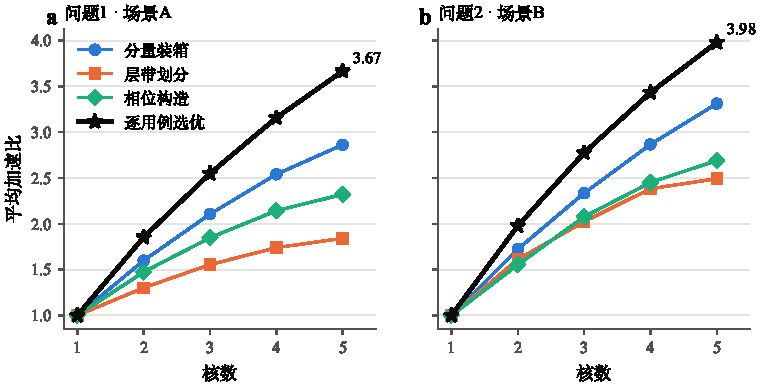
\includegraphics[width=\textwidth]{algo_compare}
  \caption{构造算法（各自在参数网格上逐用例取最优）与逐用例选优的平均加速比。(a) 问题一；(b) 问题二}
  \label{fig:algocmp}
\end{figure}

后处理中，第一轮成组合并在 \V{co1_p1_groups} 组（用例，核数）中改进了 \V{co1_p1_improved} 组，平均缩短 \V{co1_p1_mean_red_pct}，最多 \V{co1_p1_max_red_pct}；以第一轮结果为起点换用更细宽度的第二轮，\V{co2_groups} 组平均只再缩短 \V{co2_mean_red_pct}，这一方向已基本挖尽。局部搜索共运行 \V{ls_jobs_total} 个作业，每个作业的评估次数中位数 \V{ls_tries_median}、用时中位数 \V{ls_secs_median} 秒，问题一中起点可追溯的 \V{ls_p1_jobs} 个作业平均缩短 \V{ls_p1_mean_red_pct}，最多 \V{ls_p1_max_red_pct}。它的平均收益远小于换一种构造方式，我们保留它是因为在个别用例上没有替代：最终方案中问题一有 \V{source_mix_by_problem_1_localsearch} 组来自局部搜索。核数补齐在问题一中评估了 \V{mono_p1} 个补空核方案，重评后的 Makespan 与原少核方案逐个相同。补齐之后，每个用例的加速比都随核数单调不减，满足题目对 2--5 核稳定性的要求。

最终的平均加速比见图~\ref{fig:speedup}(a) 与表~\ref{tab:p1-result}：2--5 核依次为 \V{p1_k2_final_mean}、\V{p1_k3_final_mean}、\V{p1_k4_final_mean}、\V{p1_k5_final_mean}，5 核相对朴素基线（\V{p1_k5_naive_mean}）提高 \V{p1_k5_naive_gain_pct}，对含同步可达参考的平均达成率为 \V{p1_k5_achieve_mean}。2 核时有 \V{p1_k2_superlinear} 个用例 $\rho_2>2$，原因见第~\ref{sec:refs} 节：切图减少了单核基准中的换出。逐用例结果见附录 A。

上述结果用到了较大的参数网格和局部搜索，是为了尽量逼近可达水平；题目同时要求算法高效，单个用例以 5--10 分钟内给出结果为佳。为此附件程序提供快速模式：只用三种构造算法各 3 组代表参数共 9 个候选，再对其中最优者做成组合并。只看其中 9 个构造候选（尚未计入成组合并），2--5 核平均加速比已达 \V{figx_fast_p1_k2_mean}、\V{figx_fast_p1_k3_mean}、\V{figx_fast_p1_k4_mean}、\V{figx_fast_p1_k5_mean}，5 核为最终结果的九成左右。在最大的用例 case\_014（35{,}705 个操作）上，快速模式完整运行一次的 CPU 时间约 \V{figx_fast_big_cpu_min} 分钟，8 进程并行时墙钟时间约 1 分钟，其他用例更快。

\begin{figure}[H]
  \centering
  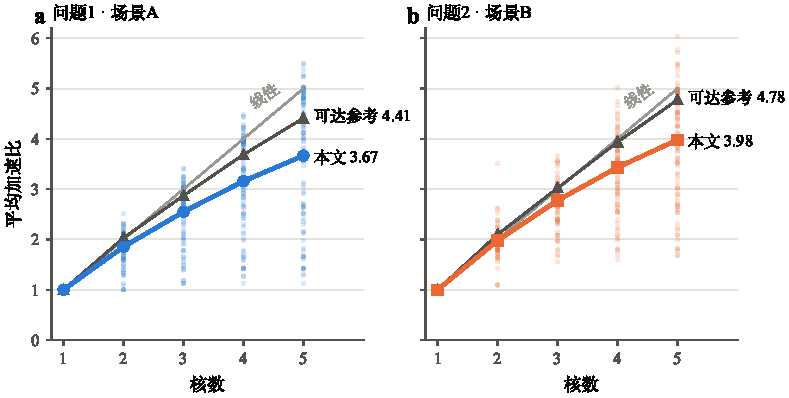
\includegraphics[width=\textwidth]{speedup_p12}
  \caption{1--5 核平均加速比（相对官方单核基准）。淡色点为逐用例加速比，三角为含同步可达参考。(a) 问题一；(b) 问题二}
  \label{fig:speedup}
\end{figure}

\begin{table}[H]
\centering
\caption{问题一结果统计（100 个用例）}
\label{tab:p1-result}
\renewcommand\arraystretch{1.15}
\begin{tabular}{lcccc}
\toprule
 & 2 核 & 3 核 & 4 核 & 5 核 \\
\midrule
平均加速比 & \V{p1_k2_final_mean} & \V{p1_k3_final_mean} & \V{p1_k4_final_mean} & \V{p1_k5_final_mean} \\
最小 / 最大加速比 & \V{p1_k2_final_min} / \V{p1_k2_final_max} & \V{p1_k3_final_min} / \V{p1_k3_final_max} & \V{p1_k4_final_min} / \V{p1_k4_final_max} & \V{p1_k5_final_min} / \V{p1_k5_final_max} \\
平均并行效率 $\bar\rho_k/k$ & \V{p1_k2_eff_mean} & \V{p1_k3_eff_mean} & \V{p1_k4_eff_mean} & \V{p1_k5_eff_mean} \\
对可达参考的达成率 & \V{p1_k2_achieve_mean} & \V{p1_k3_achieve_mean} & \V{p1_k4_achieve_mean} & \V{p1_k5_achieve_mean} \\
平均额外搬运量 / MB & \V{p1_k2_added_MB_mean} & \V{p1_k3_added_MB_mean} & \V{p1_k4_added_MB_mean} & \V{p1_k5_added_MB_mean} \\
子图数中位数 & \V{p1_k2_nsg_median} & \V{p1_k3_nsg_median} & \V{p1_k4_nsg_median} & \V{p1_k5_nsg_median} \\
超线性用例数（$\rho_k>k$） & \V{p1_k2_superlinear} & \V{p1_k3_superlinear} & \V{p1_k4_superlinear} & \V{p1_k5_superlinear} \\
\bottomrule
\end{tabular}
\end{table}

分类来看（图~\ref{fig:heatmap}），III 类 5 核平均 \V{p1_k5_famIII_mean}、达成率 \V{p1_k5_famIII_achieve}，已接近可达水平；II 类为 \V{p1_k5_famII_mean}；I 类只有 \V{p1_k5_famI_mean}，达成率 \V{p1_k5_famI_achieve}。短板集中在 I 类中规模较小的用例。case\_064 的单核基准只有 19{,}116 周期，2--5 核的最优加速比都是 1.13，多给的核心已经用不上：一次跨核等待 1000 周期，与整个计算时间同一量级，场景 A 下几乎无法从切分中获益。图~\ref{fig:bounds} 把每个用例的实测加速比与可达参考放在一起，III 类的点贴近对角线，I 类的点大多在对角线下方。

\begin{figure}[H]
  \centering
  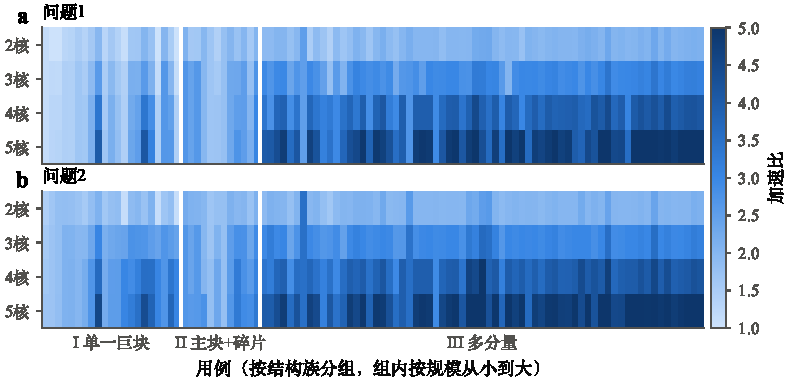
\includegraphics[width=\textwidth]{speedup_heatmap}
  \caption{逐用例加速比热力图（相对官方单核基准）。按类别分组，组内按规模从小到大排列}
  \label{fig:heatmap}
\end{figure}

\begin{figure}[H]
  \centering
  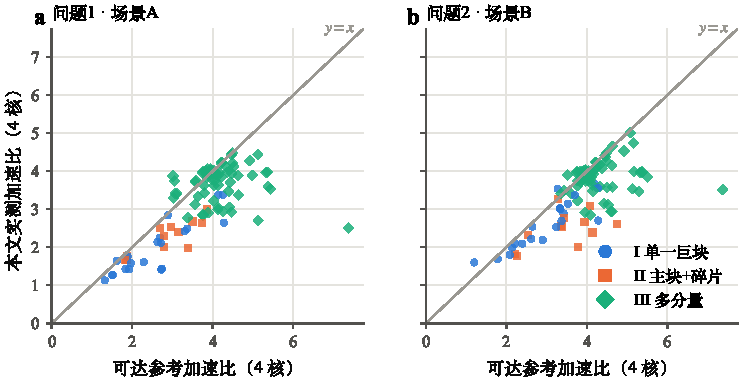
\includegraphics[width=\textwidth]{bounds_gap}
  \caption{逐用例实测加速比与含同步可达参考（4 核）。可达参考为贪心结果，少数点位于对角线上方}
  \label{fig:bounds}
\end{figure}

最终方案的来源见图~\ref{fig:wins}。问题一中成组合并是最主要的来源（\V{source_mix_by_problem_1_coarsen} 组），其次是局部搜索（\V{source_mix_by_problem_1_localsearch} 组）和相位构造（\V{source_mix_by_problem_1_phase} 组）。构造算法给出了好的起点，合并同核相邻子图、缩短依赖链上 Task 序列的后处理贡献了后一段提升。

\begin{figure}[H]
  \centering
  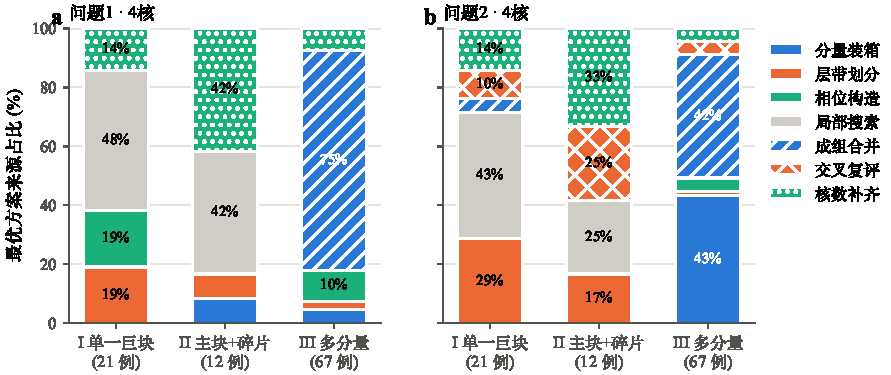
\includegraphics[width=\textwidth]{algo_wins}
  \caption{各类别中最终方案的来源（4 核）。后处理来源单独统计，不归入底层构造算法}
  \label{fig:wins}
\end{figure}

以 I 类中的 case\_002 为例看问题一的求解过程。它有 \V{cs_ops} 个可分配操作，宽度比 \V{cs_width}，单核基准 Makespan 为 \V{cs_single}。表~\ref{tab:case002-p1} 列出它在 4 核下各构造算法的最优结果。朴素分量装箱的加速比恰好为 1：整张图只有一个分量，$\alpha=0.25$ 时不被切开，全部落在一个核上。层带划分最好的 $W=\V{cs_p1_band_div}$ 也只有 \V{cs_p1_band_sp}，因为每个层带子图都是一个 Task，边界往返和激活等待抵消了并行收益。最好的构造是相位构造，且取很大的惩罚 $\lambda=\V{cs_p1_phase_div}$：这张图依赖很密，只在少数位置跨核最划算。最终方案只有 \V{cs_p1_final_nsg} 个子图，Makespan 为 \V{cs_p1_final_ms}。它的逐核时间线见图~\ref{fig:final-tl-p1}：核 0 完成主体计算后空等了近一万周期，才开始最后一个依赖其他核心结果的子图，这段空闲就是跨核激活等待与边界往返的代价，对应式 \eqref{eq:path-bound} 中的 $h\,\delta_{\mathrm{cross}}$ 项。

\begin{table}[H]
\centering
\caption{case\_002 在问题一下的结果（4 核；括号内为胜出参数）}
\label{tab:case002-p1}
\renewcommand\arraystretch{1.15}
\begin{tabular}{lcc}
\toprule
方法 & Makespan & 加速比 \\
\midrule
朴素分量装箱（$\alpha=0.25$） & \V{cs_p1_naive_ms} & \V{cs_p1_naive_sp} \\
分量装箱最优（$\alpha=\V{cs_p1_lpt_div}$） & \V{cs_p1_lpt_ms} & \V{cs_p1_lpt_sp} \\
层带划分最优（$W=\V{cs_p1_band_div}$） & \V{cs_p1_band_ms} & \V{cs_p1_band_sp} \\
相位构造最优（$\lambda=\V{cs_p1_phase_div}$） & \V{cs_p1_phase_ms} & \V{cs_p1_phase_sp} \\
最终方案 & \V{cs_p1_final_ms} & \V{cs_p1_final_sp} \\
\bottomrule
\end{tabular}
\end{table}

\begin{figure}[H]
  \centering
  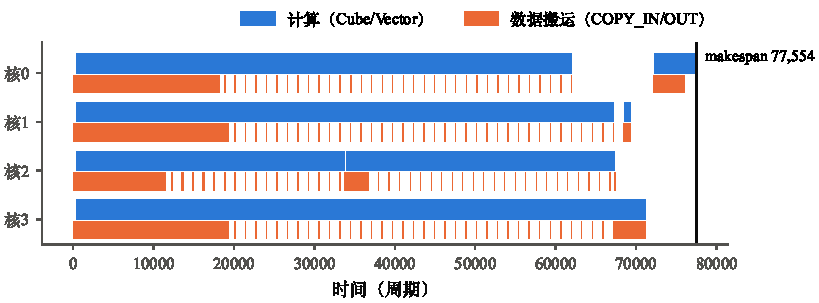
\includegraphics[width=\textwidth]{final_timeline_p1}
  \caption{case\_002 问题一最终方案（4 核）的逐核时间线。每核上条为计算流水线，下条为搬运流水线}
  \label{fig:final-tl-p1}
\end{figure}

\label{sec:neg}除上述三种构造外，实验中还否定过两条构造路线：一是把单入单出链收缩后，仍按操作粒度做通信感知表调度；二是沿最重边做链聚类，簇图成环后再做强连通缩点。为了可比，我们在每类各取 4 个、共 12 个用例上，于 4 核下与逐用例选优比较 Makespan（比值大于 1 表示更慢，取几何平均），结果见表~\ref{tab:negative}。两条路线的共同问题是子图太多，而且切断的恰恰是依赖链，商图路径因此变长，与命题~\ref{prop:path} 的判断一致。

\begin{table}[H]
\centering
\caption{未采用的构造路线（12 个用例，4 核；比值为该方法与逐用例选优的 Makespan 之比）}
\label{tab:negative}
\renewcommand\arraystretch{1.15}
\begin{tabularx}{\textwidth}{l c c c X}
\toprule
路线 & 问题 & 比值几何均值 & 最大子图数 & 失败原因 \\
\midrule
链收缩 + 表调度 & 一 & \V{neg_sched_p1_geo} & \V{neg_sched_p1_nsg_max} & 仍按操作粒度分核，子图碎成上千个，激活等待沿路径累积 \\
 & 二 & \V{neg_sched_p2_geo} & \V{neg_sched_p2_nsg_max} & 同上，跨核同步延迟累积 \\
最重边链聚类 + 缩点 & 一 & \V{neg_cluster_p1_geo} & \V{neg_cluster_p1_nsg_max} & 缩点后合法但子图仍多；仅 \V{neg_cluster_p1_nbetter} 例优于选优 \\
 & 二 & \V{neg_cluster_p2_geo} & \V{neg_cluster_p2_nsg_max} & 同上 \\
\bottomrule
\end{tabularx}
\end{table}

\label{sec:p1-check}下面检验模型本身。命题~\ref{prop:path} 断言场景 A 的代价取决于依赖路径上的子图边界，而不是子图总数。我们用两组数据检验。第一组是扫描阶段 4 核的全部 \V{figx_nsg_pairs} 个候选方案：以每个用例的最优候选为基准计算 Makespan 比值，按子图数分组取中位数（图~\ref{fig:nsg}）。问题一的曲线没有随子图数单调上升，1024 个以上子图的方案（中位 \V{figx_nsg_p1_median_5}）反而好于 16--63 个子图的方案（中位 \V{figx_nsg_p1_median_2}）；256 个以上子图的候选中约 \V{figx_nsg_hi_famIII_pct} 来自 III 类，它们切开的主要是互不相连的分量，没有拉长依赖路径。

\begin{figure}[H]
  \centering
  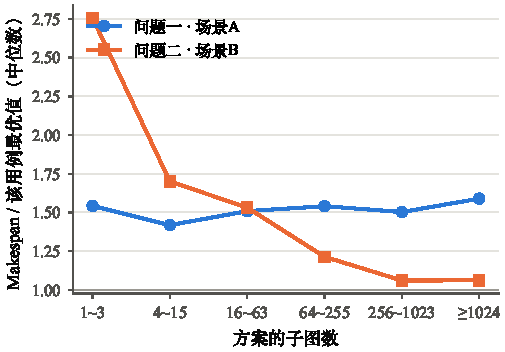
\includegraphics[width=0.66\textwidth]{nsg_quality}
  \caption{子图数与方案质量（4 核，扫描阶段全部候选）。纵轴为候选 Makespan 与该用例最优候选之比的中位数}
  \label{fig:nsg}
\end{figure}

第二组直接度量路径深度。对最终方案，在商图上按拓扑序动态规划求出最长路径上的换核次数
\begin{equation}
  h=\max_{\text{商图路径 } s_1\to\cdots\to s_m}\ \sum_{i=1}^{m-1}\chi_{s_is_{i+1}},
  \label{eq:cross-depth}
\end{equation}
其中 $\chi_{s_is_{i+1}}$ 与式 \eqref{eq:phase} 中的定义相同，相邻子图不同核时为 1。按拓扑序对每个子图记录“到达它的路径上最多换过几次核”，每条边只需做一次比较，所以一次遍历即可求出 $h$。把它与实测 Makespan 超出零通信表调度的部分对比（图~\ref{fig:depth}）。问题一中 \V{figx_depth_p1_zero} 个方案 $h=0$，即所有跨子图依赖都留在同一核心；其余方案的超出量与 $h\,\delta_{\mathrm{cross}}$ 在对数尺度上的相关系数为 \V{figx_depth_p1_corr}，全部 \V{figx_depth_p1_n} 个点都位于对角线上方，即超出量至少为 $h\,\delta_{\mathrm{cross}}$，与式 \eqref{eq:path-bound} 一致。

\begin{figure}[H]
  \centering
  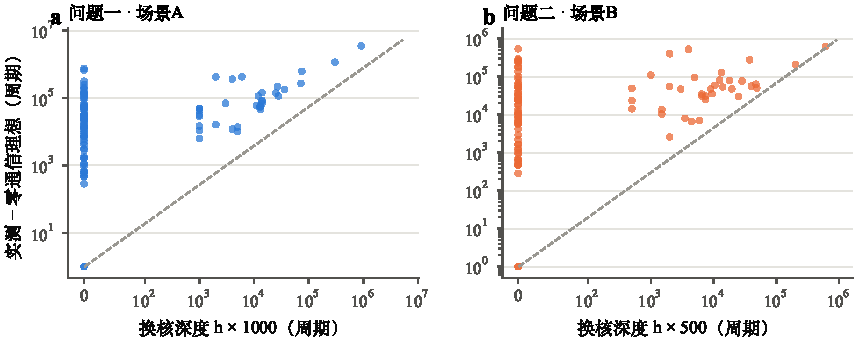
\includegraphics[width=\textwidth]{cross_depth}
  \caption{最终方案的换核深度与 Makespan 超出量（4 核）。横轴为 $h$ 乘以跨核固定延迟，纵轴为实测 Makespan 减去零通信表调度 Makespan；虚线为 $y=x$。(a) 问题一；(b) 问题二}
  \label{fig:depth}
\end{figure}
